 \section{Parser Combinators for Path Querying}

Parser combinators provide a way to specify a language syntax in terms of functions and operations on them. 
A parser in this framework is usually a function which consumes a prefix of an input and returns either a parsing result or an error if the input is erroneous. 
Parsers can be composed by using a set of parser combinators to form more complex parsers. 
A parser combinators library provides with a set of basic combinators (such as sequential application or choice), and there can also be user-defined combinators. 
Most parser combinators libraries, including the Meerkat library, can only process the linear input --- strings or some kind of streams. 
We extend the Meerkat library to work on the graph input.


\subsection{Generic interface for input}
Combinators is a way to describe a query. When we have a query we may want to execute that query on some graph considering it as an input for our query. The cool thing is that that input can be generalized to achive flexibility of all possible application of graph combinators and support a wide range of data sources. The idea is to present the input as two functions, one for working with edges and one for vertices. The first one would allow to get all edges outcoming from current vertex and also satisfies given predicate. The second one will allow to check if current vertex satisfies given predicate. That interface is presented on Fig .\ref{fig:input}. We have implementation of that input for: 
\begin{itemize}
    \item Neo4jInput --- input source for working with graph database Neo4J
    \item GraphxInput --- input source for working with graph presented in memory using GraphX library
    \item LinearInput --- input source for working with linear input data like strings
\end{itemize}

\begin{figure}[h]
\begin{lstlisting}
trait Input[+L, +N] {
  def filterEdges(nodeId: Int, 
      predicate: L => Boolean): Seq[(L, Int)]
  def checkNode(nodeId: Int, 
      predicate: N => Boolean): Option[N]
}

\end{lstlisting}
\caption{Generalized input interface}
\label{fig:input}
\end{figure}


\subsection{The set of combinators}

The basic combinators our library provides are presented in table~\ref{table:combinators}. It consists of two kind of combinators. The first kind creates new parsers from existing ones, meanwhile the second one allows mapping parsers result.
Parsers for matching strings are implicitly generated whenever a string is used within a query. 
The classical same generation query~\cite{FndDB} can be written using the library as presented in Fig.~\ref{fig:query1Meerkat}.



\begin{table}[h]
\centering
\begin{tabular}{l@{}|l}
\multicolumn{1}{c|}{Combinator} & \multicolumn{1}{|c}{Description} \\ \hline
{\lstinline!a ~ b!} & sequential parsing: {\lstinline!a!} then {\lstinline!b!}   \\
{\lstinline!a | b!} & choice: {\lstinline!a!} or {\lstinline!b!}         \\
{\lstinline!a ?!}   & optional parsing: {\lstinline!a!} or nothing   \\
{\lstinline!a *!}   & repetition of zero or more {\lstinline!a!} \\
{\lstinline!a +!}   & repetition of at least one {\lstinline!a!} \\
{\lstinline!a ^ f!} & apply {\lstinline!f!} function to {\lstinline!a!} if  {\lstinline!a!} is a token \\
{\lstinline!a ^^!}  & capture output of {\lstinline!a!} if {\lstinline!a!} is a token    \\
{\lstinline!a & f!} & apply {\lstinline!f!} function to {\lstinline!a!} if  {\lstinline!a!} is a parser \\
{\lstinline!a &&!}  & capture output of {\lstinline!a!} if {\lstinline!a!} is a parser    \\
\end{tabular}
\caption{Meerkat combinators}
\label{table:combinators}
\end{table}





\subsection{An Example}
Let's assume we have a graph which consists of cities as vertices and every cite has a name belongs to a country. There can be a road from one city to another, this relation is shown in graph as an edge with label $road\_to$. Such graph is shown on \ref{fig:graph}. Let us capture one city, let's say city $a$. Now having that graph and captured vertex we would like to know all paths such if as $i$ city from begining of our path we visit country $X$ then as $i$ city from end of our path we visit country $X$ too. And also the middle city in our path is our captured city $a$.
In a terms of combinators we can define our path as shown on Fig. \ref{fig:pathQuery}. Here \lstinline{reduceAsOr} is a function which transforms a list of queries to one query which is formed by reducing given list with \lstinline{|} combinator. The \lstinline{pathPart} combinator recursively defines a path of our way. Also, \lstinline{middleCity} is a vertex combinator which parses our captured city $a$ and \lstinline{roadTo} combinator parses a roadTo edge.

\begin{figure}[h]
\begin{lstlisting}
val countriesList = List("X", "Y")
val path = 
  (reduceAsOr(countriesList.map(pathPart)) | middleCity)
def pathPart(country: String) =
  syn(city(country) ~ roadTo ~ path ~ roadTo ~ city(country))

val middleCity = V(_.value() == "a")
val roadTo = E(_.value() == "road_to")
def city(country: String) =
  V(_.country == country)
\end{lstlisting}
\caption{Path query}
\label{fig:pathQuery}
\end{figure}


The most exciting feature of our library is that queries can be used as first-class values which means greater generalization and composition. 
The function \lstinline{reduceAsOr} presented in Fig~\ref{fig:reduceAsOr} is a generalization of bracket sequence query and is independent of the environment such as the input graph structure or other parsers.
It can be used for the creation of other queries, including the one presented in Fig~\ref{fig:pathQuery}: it is the result of the application of \lstinline{reduceAsOr} to the appropriate relations (which can be treated as opening and closing brackets).

\begin{figure}[h]
\begin{lstlisting}
def reduceAsOr(xs: List[Nonterminal]) = 
  xs match {
    case x :: Nil     => x
    case x :: y :: xs => 
      syn(xs.foldLeft(x | y)(_ | _))
  }
\end{lstlisting}
\caption{Combinators implementation}
\label{fig:reduceAsOr}
\end{figure}

Now we would like, to get from our query only \lstinline{city} combinator result. For that purpose let us modify it to make return result. In out library we have a \lstinline{^} and \lstinline{&} functions for that. Then we will have the following definition of our combinators:
\begin{figure}[h]
\begin{lstlisting}
val middleCity = 
  syn(V(_.value() == "a") ^^) & (List(_))
def pathPart(country: String) = syn(
  (city(country) ~ roadTo ~ 
    path ~ roadTo ~ city(country) & {
      case a ~ (b: List[_]) ~ Entity => 
        a +: b :+ c })
\end{lstlisting}
\caption{Fixed combinators}
\label{fig:fixedAtor}
\end{figure}

Now we execute our query. For the graph presented on fig. \ref{fig:graph} we will get paths which satisfies given criteria \lstinline{a, b->a->d, c->b->a->d->e}

A simplified SPPF for this query is presented in Fig.~\ref{fig:sppf}: rounded rectangles represent nonterminals and other rectangles represent productions. 
Every rectangle contains a nonterminal name or a production rule, as well as start and end nodes of the path in the input graph derived from the corresponding rectangle. 
Gray rectangles are start nonterminals.

\begin{figure}[h]
\includegraphics[width=0.45\textwidth]{graph}
\caption{Example Input graph}
\label{fig:graph}
\end{figure}

\begin{figure}[h]
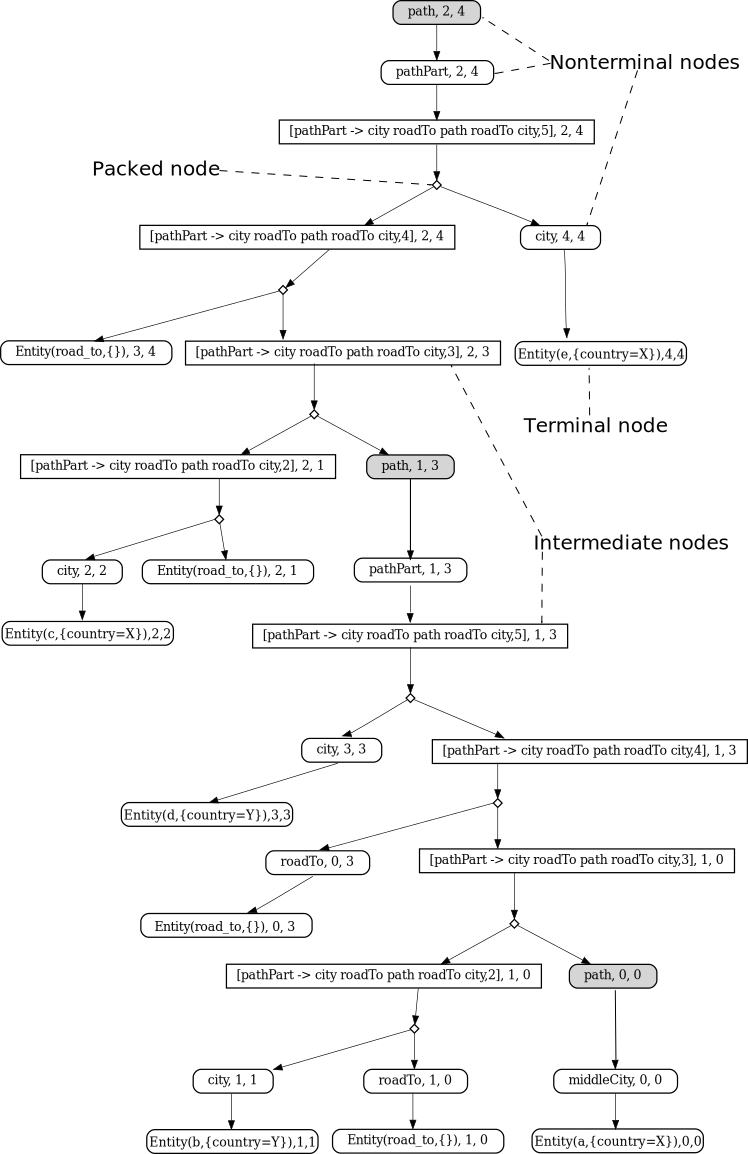
\includegraphics[scale=0.5]{sppf}
\caption{SPPF: result of applying actor/movie query to the graph~\ref{fig:graph}}
\label{fig:sppf}
\end{figure}
